% !TEX root = ../dissertation.tex

\chapter{Sancho Overview}
\label{chapter:sancho_overview}

A more up to date and detailed overview of the Sancho project is given in this chapter

\section{The overall architecture}

Sancho is based on the ggp-base framework.
It spawns many different threads but there are only 3 important types:
\begin{itemize}
	\item 1 HTTP server thread: Responsible for network communication with the game manager.
	\item 1 MCTS structure control thread: Handles all MCTS steps except simulation. It's the only thread that can modify the MCTS graph.
	\item N Playout threads: These threads handle simulations (random playouts).    
\end{itemize}
	
\todo[inline]{make diagram}
	
\begin{figure}[h]
	\centering
	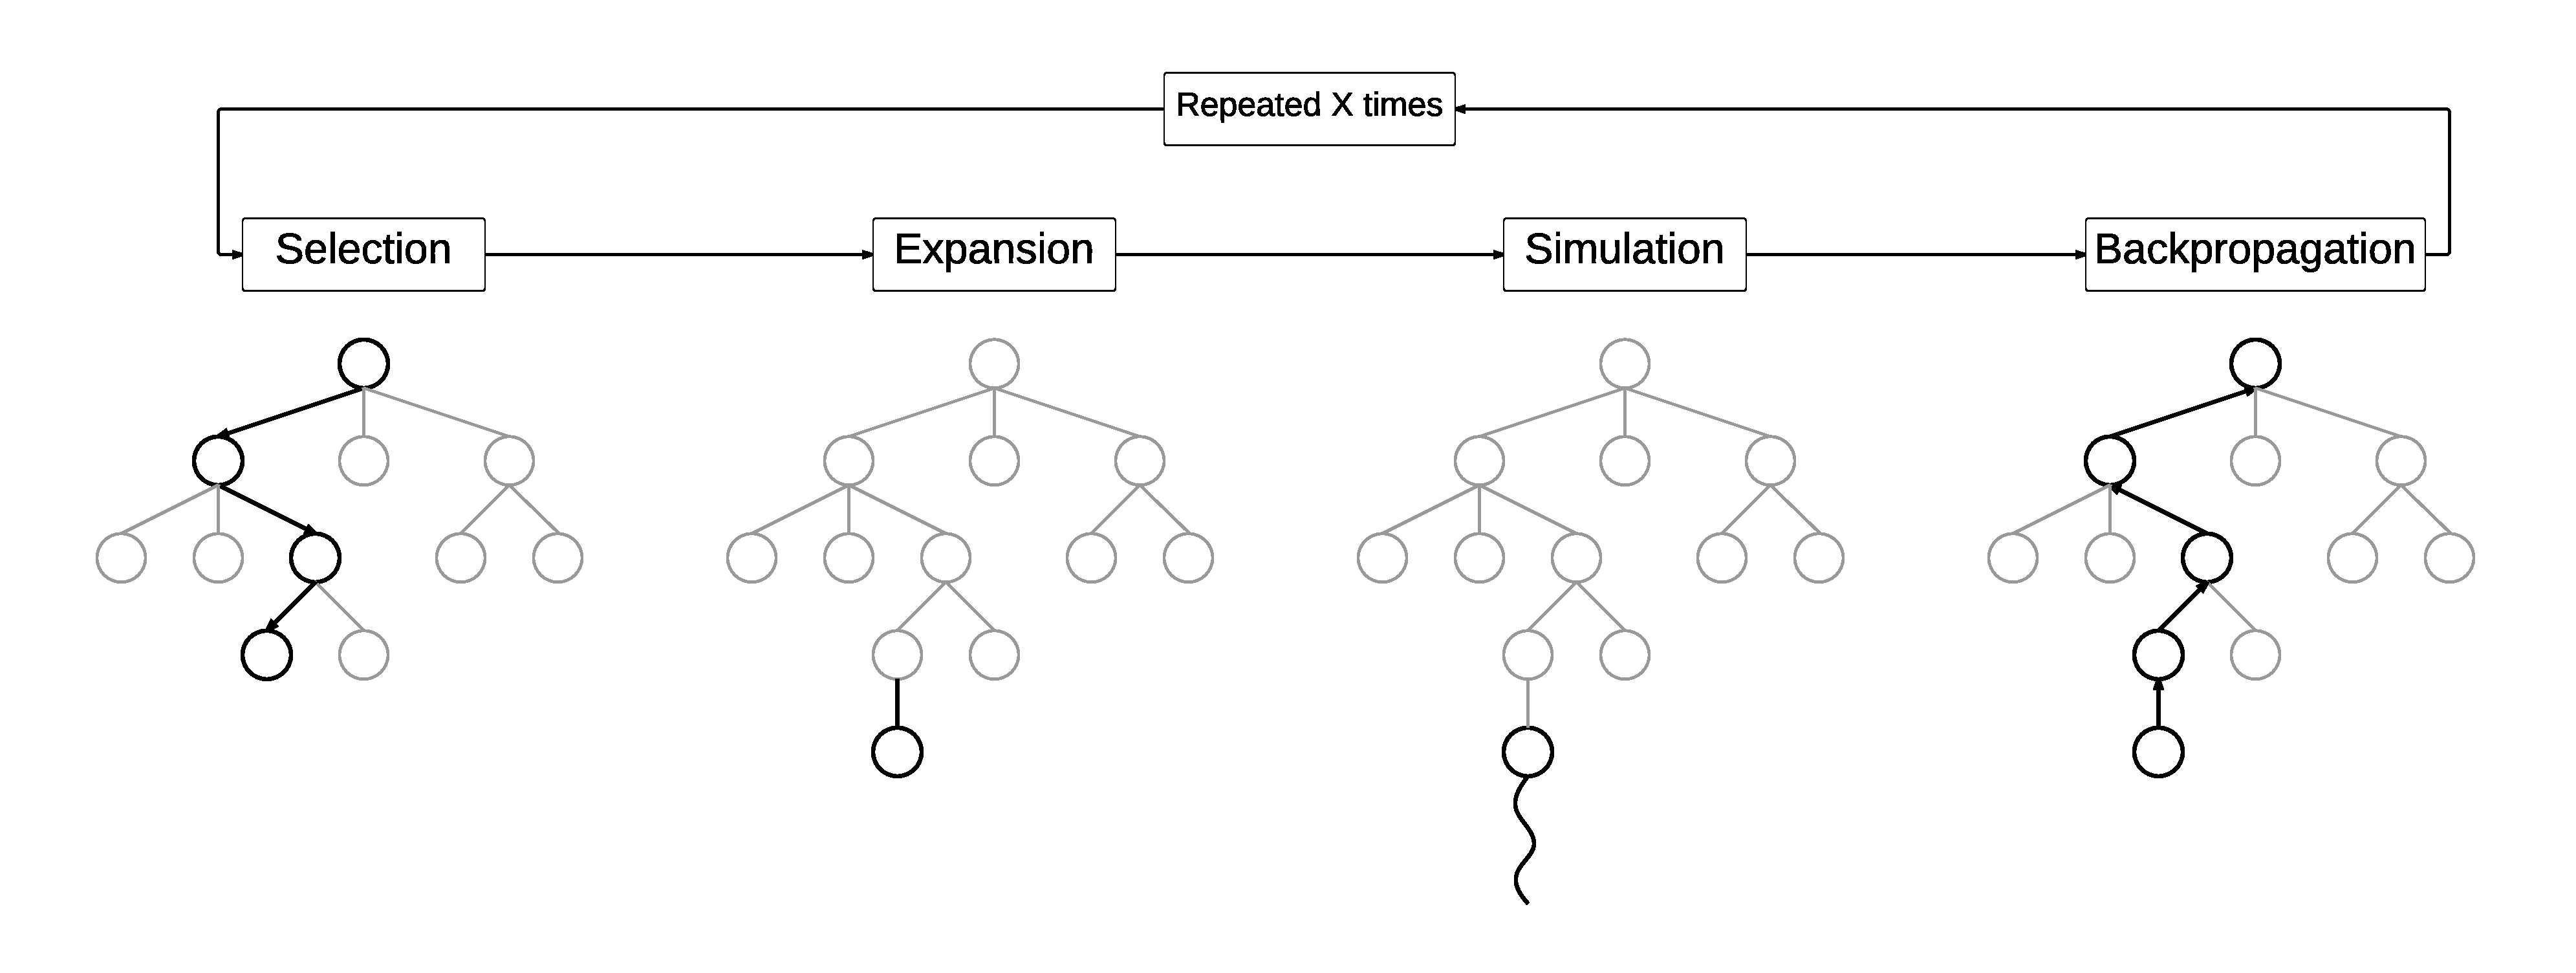
\includegraphics[width=\textwidth]{images/MCTS.pdf}
%	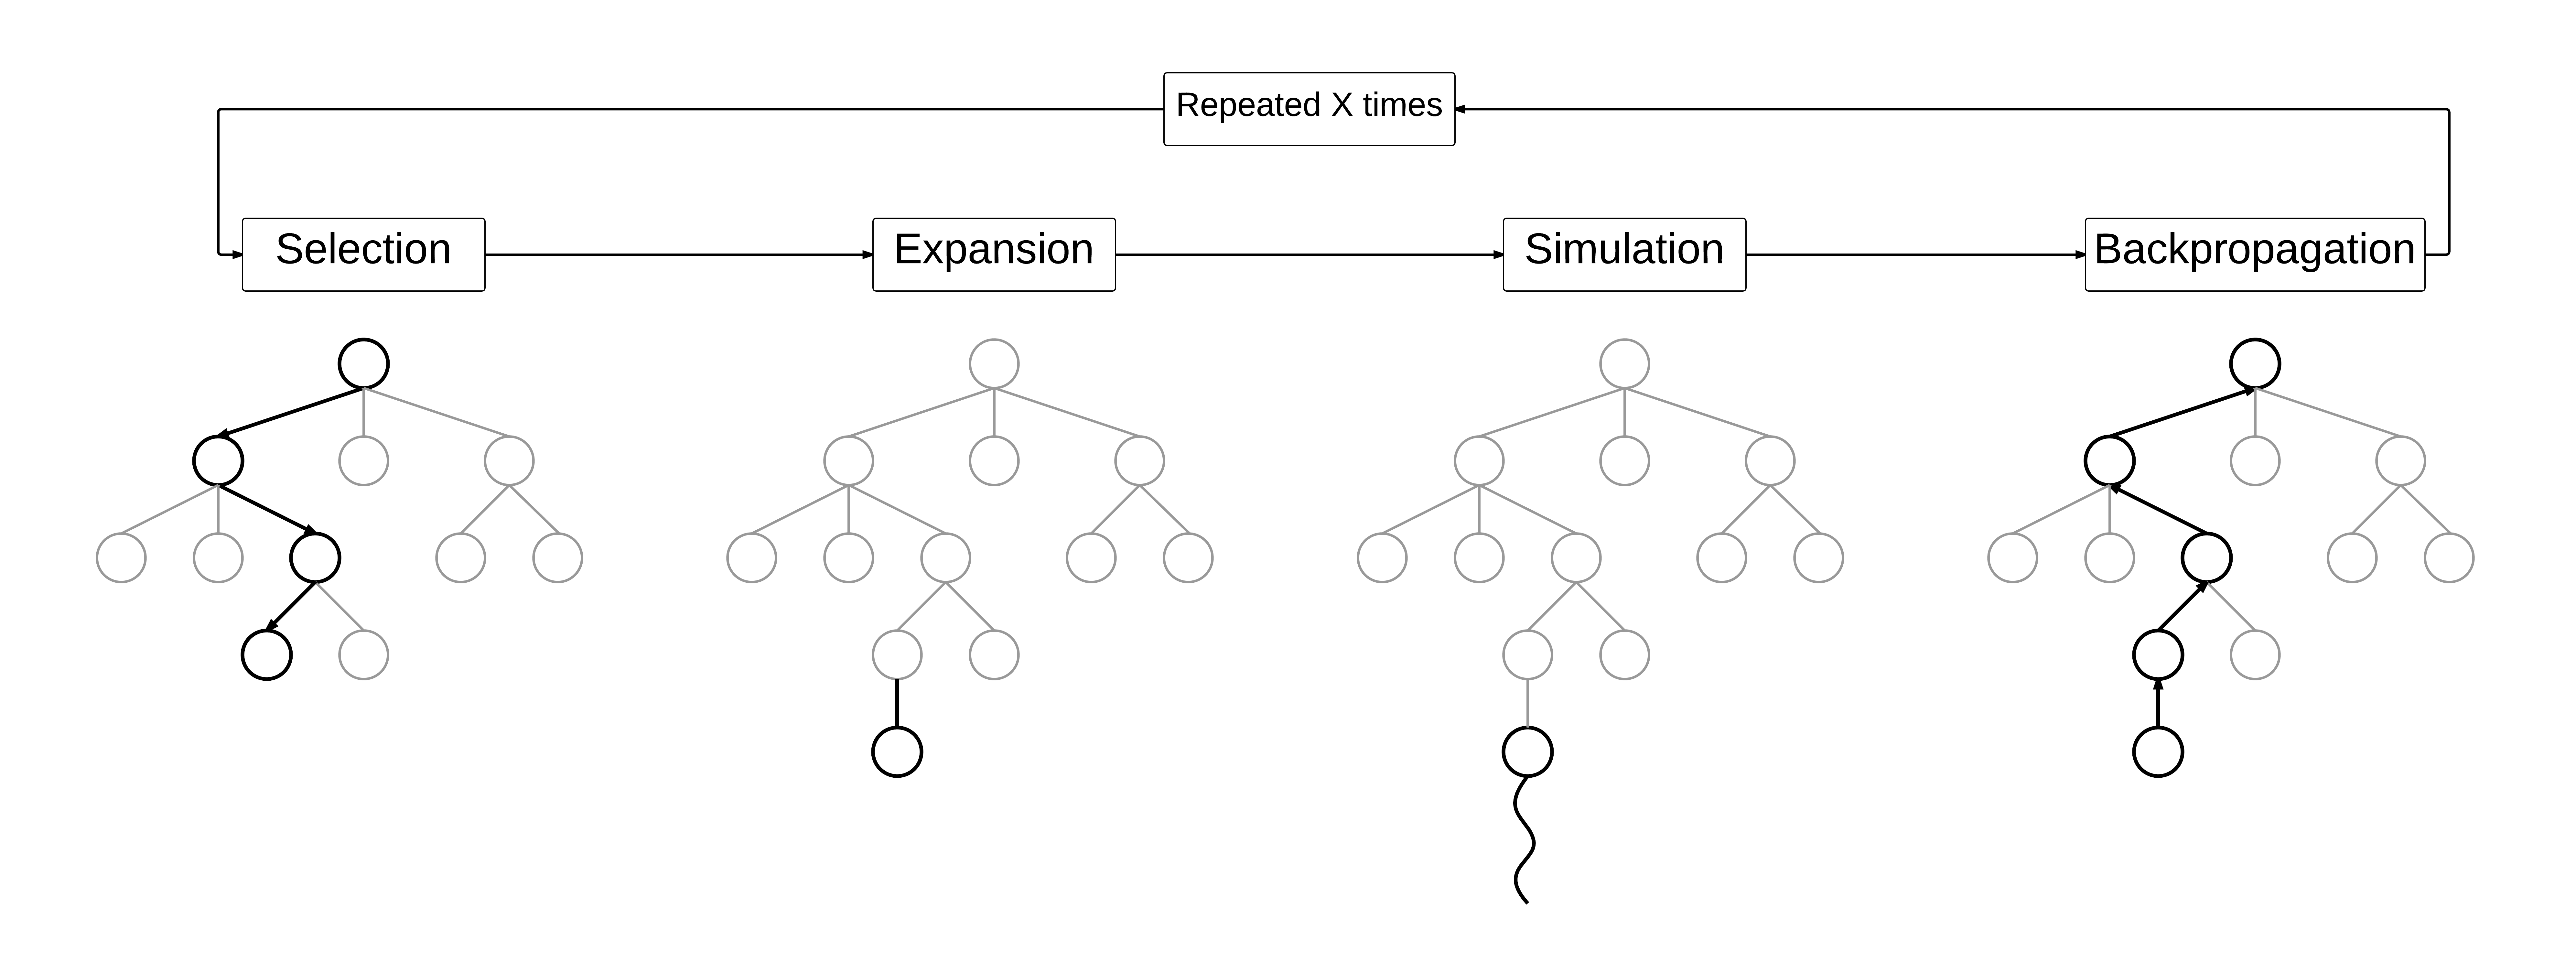
\includegraphics[width=\textwidth]{images/MCTS.png}
	\caption{MCTS steps}
	\label{fig:mcts steps}
\end{figure}

\section{MCTS data structure}
MCTS is usually done on a tree structure but Sancho uses a Directed Graph to represent the game states and transitions, allowing for each state to be represented only once, regardless of the path taken to reach it.
This has two main advantages: the values for each state can be drastically more accurate by averaging the scores from different paths and it can also save on memory.
The main drawback is making back-propagation more complicated to implement.


\section{Meta-Gaming}

\section{Heuristics}

\section{Propositional Networks Implementation}

Propositional Networks (PropNets) are used in Sancho as a faster way of computing state transitions than interpreting GDL. An example was given in  figure \ref{fig:propnets example}.
GDL can be translated into a PropNet representation since both are first order logic, GGP-base includes a GDL to PropNet converter which Sancho builds on to improve performance.

\subsection{Data Representaion}
\noindent PropNets are represented in a way that enables cheap state updates and queries:
\begin{itemize}
	\item All components store their own current state to avoid calculating state on queries. By caching the states, calculation only has to happen when a base proposition changes value.
	
	\item Logic components can have more than 2 inputs, to avoid having to represent a 5-input AND gate with 4 2-input AND gates that take up more memory and increase time complexity of propagation
	
	\item AND and OR gates store their state as an integer with a value equal to the number of inputs set to True, so that whenever one of the inputs changes, all that has to be done to calculate the new output is to increment or decrement the integer and do a simple if statement. (This is actually done a bit more efficiently but the idea is very similar)
	
	\item PropNet state (values of components) and structure (component type and connections) are stored separately, so that multi-threading is possible: the PropNet structure is shared and read-only and each thread stores it's own version of PropNet state, so that no blocking is needed. These threads can then be used to calculate different state-transitions in parallel. More details about how this is stored are given below.
\end{itemize}

The PropNet structure itself (what components exist and what they're connected to) is stored in two fixed length arrays, as can be seen in \ref{fig:propnet_structure}.
PropNet states are also stored in fixed length arrays, where each entry is the value of a base proposition of the net.

Note: During the creation and optimization process of the propnet Sancho actually uses more dynamic and high-level data structures from Java's collections. When the final topology is reached the conversion to these low-level/high-performance data structures is done.
	
\begin{figure}[h]
	\centering
	\includegraphics[width=0.75\textwidth]{images/PropNet_Structure.pdf}
	\caption{Propositional Network structure}
	\label{fig:propnet_structure}
\end{figure}

\subsection{Further optimizations}
After the initial GDL to PropNet translation is done Sancho tries several methods of improving the performance of the network:
\begin{itemize}
	\item Several techniques are used to try to reduce the number of components, like doing associative, distributive and DeMorgan's transformations and removal of redundant components (like two NOT gates in series) and duplicate components.
	
	\item Moving goal score calculation to a separate network since it's only relevant on terminal states, so it's ok to calculate it's values from scratch when needed (by querying the current values of the main network) because it's rarely needed.
	
	\item Whenever a component changes value it forces a recalculation on all components that it outputs to,  initiating a forward-propagated update of the PropNet.
	It's actually a differential forward propagation, since components only propagate updates if their own outputs change
	
	\item When possible, factor the network into multiple independent sub-networks. This happens with compound games (n independent games glued together) and is a big win in performance because it reduces the branching factor to a+b instead of a*b, where a is the branching factor for one game and b for the second (there can of course be more than 2)
	
	\item Moving control logic (like the logic that calculates whose turn it is) out of the PropNet and converting it into functions like counters
	
\end{itemize}



\section{1-player games (puzzles) solving}




